% *********************************************************************
% © 2026 Jeremy Sylvestre
%
% Permission is granted to copy, distribute and/or modify this document
% under the terms of the GNU Free Documentation License, Version 1.3 or
% any later version published by the Free Software Foundation; with no
% Invariant Sections, no Front-Cover Texts, and no Back-Cover Texts. A
% copy of the license is included in the appendix entitled “GNU Free
% Documentation License” that appears in the output document of this
% PreTeXt source code. All trademarks™ are the registered® marks of
% their respective owners.
%
% *********************************************************************
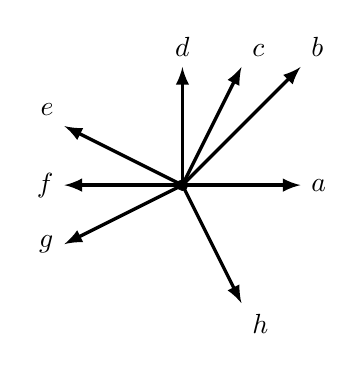
\begin{tikzpicture}[
	vector/.style={-latex,very thick},
	point/.style={circle,draw,very thin,fill,inner sep=0pt,minimum size=4pt},
	scale=0.75
]
	\coordinate (o) at ( 0, 0);
	\coordinate (a) at ( 2, 0);
	\coordinate (b) at ( 2, 2);
	\coordinate (c) at ( 1, 2);
	\coordinate (d) at ( 0, 2);
	\coordinate (e) at (-2, 1);
	\coordinate (f) at (-2, 0);
	\coordinate (g) at (-2,-1);
	\coordinate (h) at ( 1,-2);

	\node[point] at (o) {};

	\draw[vector] (o) to (a) node[right]       {$\uvec{a}$};
	\draw[vector] (o) to (b) node[above right] {$\uvec{b}$};
	\draw[vector] (o) to (c) node[above right] {$\uvec{c}$};
	\draw[vector] (o) to (d) node[above]       {$\uvec{d}$};
	\draw[vector] (o) to (e) node[above left]  {$\uvec{e}$};
	\draw[vector] (o) to (f) node[left]        {$\uvec{f}$};
	\draw[vector] (o) to (g) node[left]        {$\uvec{g}$};
	\draw[vector] (o) to (h) node[below right] {$\uvec{h}$};

\end{tikzpicture}
